\chapter{A fejlesztés folyamata}

A teljesítmény elektronikai eszközök fejlesztésének a nehézsége abban rejlik, hogy a kisebb teljesítményű modell nem feltétlenül viselkedik úgy, mint nagy áramú társa. A fenti leíráson az is jól látszik, hogy bizonyos folyamatok párhuzamosíthatóak. A szoftver fejlesztés elkezdődhet a nagy áramú elektronika tervezésével együtt, illetve a vezérlő elektronikák is tervezhetőek a kezdeti specifikációk, illetve a a kapcsolódási pontok definiálása után. A fejlődő szoftver teszteléséhez azonban elengedhetetlen, hogy a beágyazott eszköz megkapja a szükséges gerjesztéseket a külvilágtól. Amíg nem áll rendelkezésre a valós eszköz, addig ezt egy szimulátorral vagyunk kénytelenek megvalósítani. Ez lehet akár egy Hardware-in-the-Loop szimulátor. Egy ilyen eszköz jól jön azonban amikor már a valós frekvenciaváltó is rendelkezésre áll. Az egyes szoftver módosításokat célszerű kipróbálni ezen az eszközön először, mert egy hiba könnyedén végzetes következményekkel járhat a valós inverteren.  \cite{sutozoli}

\section{Különböző szimulációs eljárások összehasonlítása}

\paragraph{}
Jól látható tehát, hogy egyértelmű igény mutatkozik valamilyen szimulációs eljárás használatára a fejlesztés minden szakaszában. Természetesen mint minden problémánál, itt is több megközelítés közül választhatunk. Ami mindenképp közös az eljárásokban, hogy a kiváltott hardver-elemek matematikai modelljeit fel kell állítani, azok helyességéről meg kell győződni. A modellezés pontossága és az erőforrás igény között azonban meg kell találni az adott alkalmazásnak és annak szükségleteinek megfelelő kompromisszumot. Elengedhetetlen követelmény azonban, hogy az irányító elektronika szempontjából a modell teljesen transzparens legyen, egyébként nem tudunk reprezentatív következtetést levonni a működés helyességével kapcsolatban. Ez azt jelenti, hogy ugyan azokon az interfészeken keresztül tudjunk a szimulátorral interakcióba lépni, ugyan azokat a válaszokat kapja a szakasztól, mint amit a valóságban is fog kapni, valamint az időzítések is egyezzenek meg az igazi eszközön tapasztaltakkal.

\paragraph{}
Joggal merül fel a gondolat, hogy asztali számítógépen futtassuk a kifejlesztett modellt, hiszen szokványosan használjuk PC-nket különböző számítások elvégzésére. Ezzel módszerrel azonban nagyon hamar problémákba ütközünk. Az első követelmény, hogy rendelkezzen a számítógépünk adat gyűjtő modullal (DAQ - Data Aqusition Module), mely segítségével tudunk mérni és előállítani analóg és digitális jeleket. Ilyen eszközöket lehet kereskedelmi forgalomban kapni, kérdéses azonban a biztosított sávszélesség, a számítógéppel való kommunikáció sebessége, illetve a költsége a vásárolt hardvernek. Ezen felül korlát még az időzítések betartása. Nem is biztos, hogy a számítógépünk valós időben el tudja végezni a szimulációhoz szükséges matematikai műveleteket, de ha feltételezzük, hogy igen, az egzakt és konzisztens lépésköz egy általános célú asztali számítógépen nem garantálható az operációs rendszer sajátságaiból adódóan. Ennek megoldására állnak rendelkezésre valós idejű megoldások, például valós idejű futást támogató Linux kernel, melyet hasonló célra fejlesztettek ki. A számítógép hardveres konfigurációja is korlátot jelent, mert hiába növeljük a processzor teljesítményt, egy ponton túl ($1 - 10 \mu{}s$) a memória hozzáférések késleltetése miatt nem tudunk kisebb szimulációs lépésközt biztosítani.

\paragraph{}
A következő lehetőség saját beágyazott hardver fejlesztése, mely emulálja a valós teljesítmény elektronikát. Ebben az esetben teljesen testre tudjuk szabni a kapcsolódási pontokat, elő tudjuk állítani azokat a jeleket, melyeket vár a vezérlő elektronika, pontosan úgy ahogy szeretnénk. Előnye a beágyazott processzornak, hogy architektúrájából adódóan garantált futásidőt lehet elérni. A teljesítménye azonban korlátozott az asztali számítógéphez képest, bár, mivel csak egy specifikus feladatot kell végrehajtani, akár még versenyezhet is futásidőben az asztali számítógéppel. Fentiek miatt ez a megoldás leginkább funkcionális tesztek végrehajtására alkalmas, precíz, kvantitatív tesztek végzésére korlátozottan.

\paragraph{}
A harmadik út - amit részletesebben megvizsgálok dolgozatomban - az FPGA alapú hardware-in-the-loop szimulátor tervezése. Bár a fejlesztési idő és a hardver költsége szintén magas lehet, az FPGA architektúrájából adódóan, nevezetesen, hogy létre tudjuk benne hozni az éppen szükséges számításokat elvégző hardvert, rendkívül gyors futásidő érhető el. Ráadásul a PC-vel ellentétben itt az FPGA teljesítményének és órajelének növelésével egyre nagyobb felbontású szimulációt érhetünk el, de már a mai technológia is $100 - 10 \ ns$ futásidőre képes.

\begin{figure}[h]
	\centering
	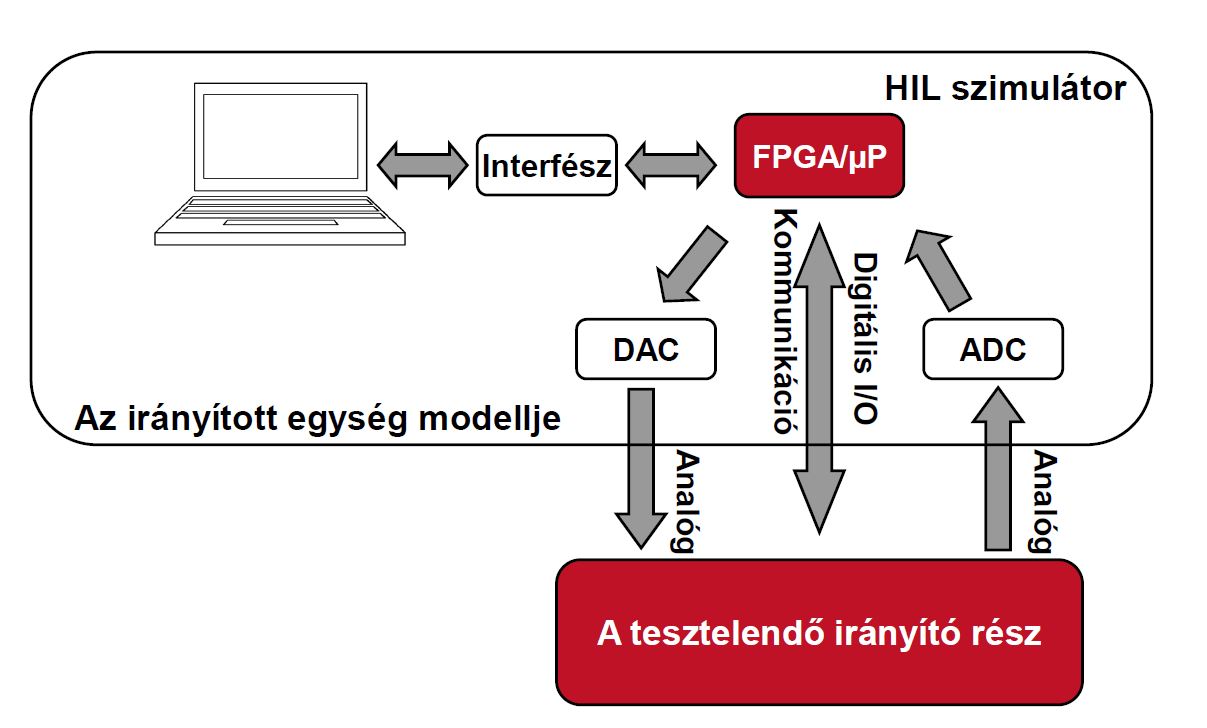
\includegraphics[width = 0.8\textwidth]{figures/hil_idea.png}
	\caption{Az FPGA alapú HIL szimulátor felépítése \cite{kokippt}} 
	\label{fig:hil_idea}
\end{figure}

\section{Szimulációs algoritmusok\cite{koki_varjasi}}

Az áramköri szimulációk numerikus megoldása általában differenciálegyenlet rendszerekre vezethetőek vissza. Az irodalom számos megoldásról említést tesz. A legtöbb eseteben a modellezendő szakasz matematikai modelljét felállítjuk egy ismert gerjesztésre adott válasz alapján, majd az így kapott modellt diszkretizáljuk.

Egy általános folytonos idejű rendszert az alábbi egyenletek reprezentálnak: 

\begin{equation}
\begin{align*}
\underline{x}'(t) &= \underline{\underline{A}}\cdot \underline{x}(t) + \underline{\underline{B}}\cdot{}\underline{x}(t) \\[0.3em]
\underline{y}(t) &= \underline{\underline{C}}\cdot \underline{x}(t) + \underline{\underline{D}}\cdot{}\underline{x}(t)
\end{align*} 
\end{equation}

ahol, $\underline{x}$ az állapotváltozók vektora, az $\underline{u}$ a rendszer bemenete, $\underline{y}$ pedig a rendszer által adott válasz.
A legegyszerűbb numerikus megoldó módszer az Euler módszer, mely az állapot változók módosításán alapul, minden lépésben maguk az állapot változók és a bemenet aktuális értéke alapján. A diszkretizált egyenlet rendszer az előrelépő (forward) Euler módszert alkalmazva az alábbi alakot ölti:

\begin{equation}
\begin{align*}
\underline{x}[n + 1] &= (\underline{\underline{A}} \cdot T + \underline{\underline{I}}) \cdot \underline{x}[n] + \underline{\underline{B}}\cdot{}T\cdot{}\underline{x}[n] \\[0.3em]
\underline{y}[n] &= \underline{\underline{C}}\cdot \underline{x}[n] + \underline{\underline{D}}\cdot{}\underline{x}[n]
\end{align*} 
\end{equation}

ahol $\underline{\underline{I}}$ az egység mátrix, $T$ a lépésköz, $n$ pedig az aktuális lépés indexe.Egy másik változata az Euler módszernek a hátralépő (backward) Euler módszer, vagy más néven implicit Euler módszer. A különbség a két módszer között, hogy az implicit Euler az aktuális értékek helyett a következő lépés értékeit használja:

\begin{equation}
\underline{x}[n + 1] = \ x[n] + \underline{\underline{A}} \cdot T \cdot \underline{x}[n + 1] + \underline{\underline{B}}\cdot{}T\cdot{}\underline{u}[n+1] \\[0.3em]
\end{equation}

Mivel $\underline{x}[n+1]$ az egyenlet mindkét oldalán megjelenik, implicit módszerről beszélünk. Átrendezés után az állapot egyenlet az alábbi alakot öltik:

\begin{equation}
\begin{align*}
\underline{x}[n + 1] &= (\underline{\underline{I}} - \underline{\underline{A}} \cdot T )^{-1} \cdot\underline{x}[n] + (\underline{\underline{I}} - \underline{\underline{A}} \cdot T)^{-1} \underline{\underline{B}}\cdot{}T\cdot{}\underline{x}[n + 1] \\[0.3em]
\underline{y}[n] &= \underline{\underline{C}}\cdot \underline{x}[n] + \underline{\underline{D}}\cdot{}\underline{x}[n]
\end{align*} 
\end{equation}

A formulából jól látszik, hogy az aktuális érték kiszámításához szükség van a változók ,,jövőbeni'' értékére. Erre következtethetünk a változók jelenlegi értékéből, vagy további késleltetést adva a rendszerhez összegyűjthetjük a számításhoz szükséges értékeket.
A két korábbi módszer kombinációja, mely széles körben alkalmazott szimulációs eljárások során a következő. Ez a módszer a trapéz módszer, a változók jelenlegi és következő lépésbeli értékek átlagát használja, így jobb közelítést adva, mintha két korábbi értéket használna:

\begin{equation}
\underline{x}[n + 1] = \ x[n] + \frac{1}{2}\underline{\underline{A}} \cdot T \cdot \underline{x}[n + 1] + \frac{1}{2}\underline{\underline{A}}\cdot{}T\cdot{}\underline{x}[n] + \frac{1}{2}\underline{\underline{B}} \cdot T \cdot \underline{u}[n + 1] + \frac{1}{2}\underline{\underline{B}}\cdot{}T\cdot{}\underline{u}[n] \\[0.3em]
\end{equation}

\paragraph{}
Látható, hogy ez szintén egy implicit módszer, hiszen ez is tartalmazza $\underline{x}[n+1]$-et mindkét oldalon, illetve szintén támaszkodik a gerjesztés jövőbeni értékére is. Kifejezve $\underline{x}[n+1]$-et az alábbi alakot kapjuk:

\begin{equation}
\begin{align*}
\underline{x}[n + 1] &= (\underline{\underline{I}} - \frac{1}{2}\underline{\underline{A}} \cdot T )^{-1} \cdot{} (\underline{\underline{I}} + \frac{1}{2}\underline{\underline{A}} \cdot T )^{-1} \cdot{} \underline{x}[n] + (\underline{\underline{I}} - \frac{1}{2}\underline{\underline{A}} \cdot T)^{-1} \cdot{} \\ (\frac{1}{2}\underline{\underline{B}} \cdot{} T \cdot{} \underline{u}[n+1] + \frac{1}{2}\underline{\underline{B}} \cdot{} T \cdot{} \underline{u}[n])  \\[0.3em]
\underline{y}[n] &= \underline{\underline{C}}\cdot \underline{x}[n] + \underline{\underline{D}}\cdot{}\underline{x}[n]
\end{align*} 
\end{equation}

\paragraph{}
Az összes módszer mátrix műveletekre vezethető vissza, az implementációjukhoz csupán mátrix szorzásra és összeadásra van szükség. Egy olyan szimulátor, amely általános állapot egyenletek megoldására képes, igen rugalmas tud lenni, a mátrixok együtthatóinak változtatásával, különböző rendszerek szimulációit hozhatjuk létre. További numerikus integráláson alapuló algoritmusok is állnak rendelkezésre, de ezek már másodrendű módszerek, amely azt jelenti, hogy szükségük van az állapot változók.
\paragraph{}
Szintén gyakran használt közelítő algoritmus a negyed rendű Runge-Kutta módszer, mely a numerikus integrálástól eltérő megközelítést alkalmaz.

\begin{equation}
\begin{align*}
\underline{a}[n] &= \underline{\underline{A}}\cdot \underline{x}[n] + \underline{\underline{B}}\cdot{}\underline{u}[n] \\[0.3em]
\underline{b}[n] &= \underline{\underline{A}}\cdot (\underline{x}[n] + \frac{1}{2}T \cdot \underline{a}[n]) + \underline{\underline{B}}\cdot{}\underline{x}[n + 0,5] \\[0.3em]
\underline{c}[n] &= \underline{\underline{A}}\cdot (\underline{x}[n] + \frac{1}{2}T \cdot \underline{b}[n]) + \underline{\underline{B}}\cdot{}\underline{x}[n + 0,5] \\[0.3em]
\underline{d}[n] &= \underline{\underline{A}}\cdot (\underline{x}[n] + T \cdot \underline{c}[n]) + \underline{\underline{B}}\cdot{}\underline{x}[n + 1] \\[0.3em]
\underline{x}[n+1] &= \underline{x}[n] + \frac{1}{6}T \cdot{} (\underline{a}[n] + 2 \cdot{} \underline{b}[n] + 2 \cdot{} \underline{c}[n] + \underline{d}[n]) \\[0.3em]
\underline{y}[n] &= \underline{\underline{C}} \cdot{} \underline{x}[n] + \underline{\underline{D}} \cdot \underline[n]
\end{align*} 
\end{equation}

ahol $\underline{a}$, $\underline{b}$, $\underline{c}$, és $\underline{d}$ csak ideiglenesen használt vektorok. Ennek az algoritmusnak nem csak a gerjesztés következő értékére, hanem a két lépés közötti ($\underline{u}[n+0,5]$), melyet könnyedén megoldhatunk a bemenet kétszeres frekvenciájú mintavételezésével, vagy a két egymást követő érték átlagának kiszámításával.